\documentclass{article}

% Language setting
% Replace `english' with e.g. `spanish' to change the document language
\usepackage[english]{babel}

% Set page size and margins
% Replace `letterpaper' with`a4paper' for UK/EU standard size
%\usepackage[letterpaper,top=4cm,bottom=4cm,left=3cm,right=3cm,marginparwidth=1.75cm]{geometry} % če to zakomentiram pride bolj ozko

% Useful packages
\usepackage{amsmath}
\usepackage{listings}
\usepackage{amssymb}
\usepackage{amsfonts} 
\usepackage{graphicx}
\usepackage{subfigure}
\usepackage{tikz}
\usepackage{graphicx}
\usepackage[T1]{fontenc}
\usepackage[colorlinks=true, allcolors=blue]{hyperref}


\newcommand{\twopartdef}[4]
{
	\left\{
		\begin{array}{ll}
			#1 & \mbox{if } #2 \\
			#3 & \mbox{if } #4
		\end{array}
	\right.
}




\title{%
The evasion problem \\
\large Computational topology -- Project}
\author{Barbara Lipnik, Evgenija Burger}

\begin{document}
\maketitle

%\abstract{abstract}

\section{Introduction}
Imagine we have a room covered with moving sensors. Our goal is to find out if there's a way for an intruder to move around this room without getting detected by any of the sensors. With some simplifications we will explore the room and how the sensors are positioned at different times and then try to find the answer to the problem with the help of persistence topology. 


\section{Problem description}
Let's have a room in the shape of a rectangle with a fixed number of sensors. Each sensor covers 4 tiles in the room and moves with a constant speed in straight lines of a fixed distance.

\begin{figure}[!h]
    \centering
    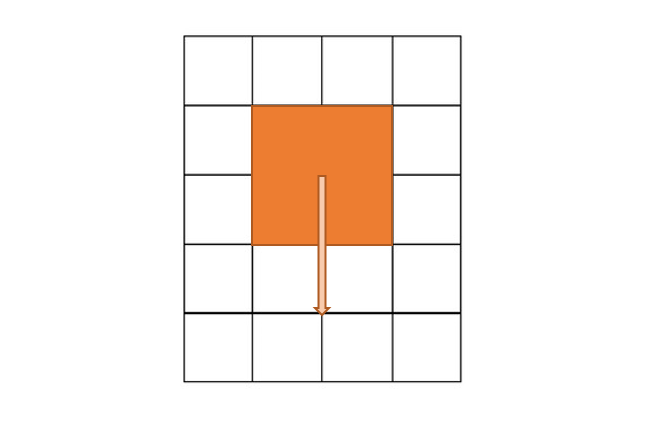
\includegraphics[width=0.5\textwidth]{sensors}
    \caption{Representation of the movement of the sensor.}
    \label{fig:sensors}
\end{figure}

 First thing we notice is that the room will eventually ``reset'' itself and come back to its starting position since the movement of all sensors is periodic. This time period $p$ can be easily calculated as the lowest common multiplier of all sensor time periods. This also means that we can describe the exact position of each sensor  and create snapshots of a room for every $t$ between 0 and $p$. Since the sensors move continuously from point to point we can connect the two different positions of a sensor between two consecutive snapshots. This will form a 3 dimensional prism. 
 
 \begin{figure}[!h]
    \centering
    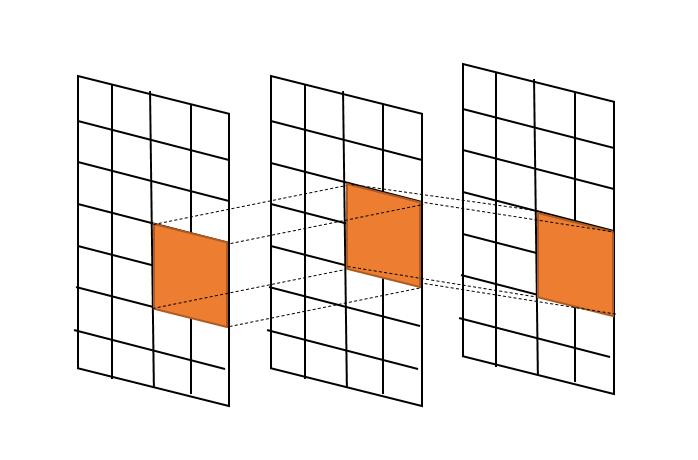
\includegraphics[width=0.7\textwidth]{complex}
    \caption{Representation of the prisms between snapshots of the room.}
    \label{fig:complex}
\end{figure}
 
 If we do this for all sensors and all times between 0 and $p$ and combine them together we will get a covered complex $C$. We already established that the movement around the room is periodic so we can glue the first and the last snapshot together so that the complex will resemble a torus. 

So what we are actually trying to find is a path around and through this torus which would represent the path the intruder could take in order for him not to get detected by any of the sensors. 




\section{Solution}

%\begin{enumerate}
%\item 
%
%\end{enumerate}

Firstly we had to find a way to describe the complex. We decided to work with cubical complexes instead of simplicial. To construct the complex and compute necessary things we used  programming language Python as we were familiar with it, its simple to use and has some useful libraries for our needs. In particular we used the Gudhi library for calculating the homology and constructing the complex. We got the answer to our problem by computing persistence homology of the cubical complex and then filter out the homologies we were interested. More about how we implemented it and how we found the right homologies is described in the next section.

A big part of our project were also the animations of the room and the moving sensors which helped with the visualization of the problem. 

Lastly we wanted to see if there's a way for us to find the path the intruder could take to not get detected. To do this we would need to find homology generators. Unfortunately the Gudhi library doesn't offer a way to compute them for periodic cubical complexes which would mean we would have to implement the functions ourselves and this would quickly expand to a broader problem that is not essential to our project.  We did try an alternative method which had nothing to do with topology but was a fun idea we wanted to play with. Firstly we talked about creating an algorithm that finds all possible paths from intruder's starting position but we quickly realized this would take long for bigger rooms and fewer sensors. So we created an algorithm that tries to find a path randomly (which is perhaps something an intruder would try). This is described in one of the following sections.

\section{Code overview}
In this section we will take a look at the code and its organisation. 


Our code is structured in a few different files where \texttt{main.py} is the main file to run the animation and outputs results. 

\subsection*{Sensors and rooms}

File \texttt{room.py} contains two classes that represent sensors and the whole room. The room is presented as a two dimensional matrix that has zeros on unsupervised cells and ones where it is scanned by sensors. A single sensor has four attributes. These are \textit{position} on the grid created by the room, its \textit{direction} and two integers \textit{steps\_forward} and \textit{steps\_back}. Those are numbers of steps the sensor can make in each direction from the current position. With this information the sensor and all its movement is fixed. The Room class has some methods that compute the period, the time slices at desired time and methods for creating a cubical complex. Depending on the optional argument the method \textit{create\_complex()} creates a periodic cubical complex using filtration numbers of each cube. The filtration is set such that at each time unit we add a new layer to the complex. This layer is the time slice of the room. If the parameter \textit{covered} is set to True, a complex representing the covered region is created. Otherwise we create a complex of the uncovered region, which is more useful for the analysis. 


\subsection*{Finding the homologies}

File \texttt{room\_operations.py} contains functions that give us some information about the room. For instance we have a function \textit{whole\_room\_supervised()} that checks if every part of the room is covered by sensors at least some of the time. Then we have \textit{one\_dimensional\_loop()} that basically returns the solution of the evasion problem for the given room. It computes the periodic cubical complex and its persistence homology. Then it filters out appropriate one dimensional homologies. As the shape of the room si essentially a torus, we can get many different $1$-dim homologies, but not all of them represent the problem solutions. As seen on figure \ref{fig:torus}, the red loop does not give us a solution to our problem. Because we used filtration based on time, we know that at time equal to the period (to be exact, to period minus one, as we start counting time with zero) the complex connects to a torus. So every homology with birth time before that must be of the same type as the red one on the figure and is as such, not a solution. Therefore we only keep homologies that were created at the time equal to the period. Function \textit{one\_dimensional\_loop()} does this filtrating. If none path is found, the function returns $[(-1, -1)]$ indicating there is no way for an intruder to stay in the room unnoticed.
All the information about the room is then printed using function \textit{compute\_homology()}.

\begin{figure}[!h]
    \centering
    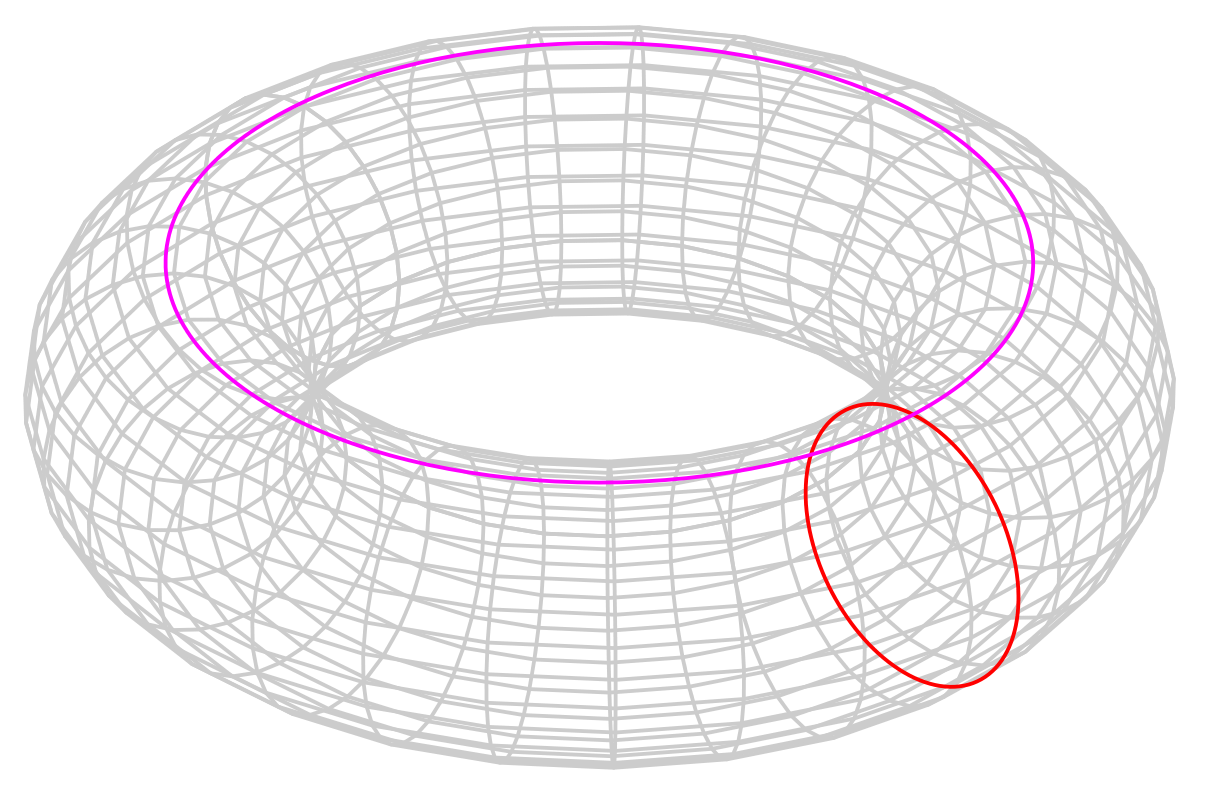
\includegraphics[width=0.5\textwidth]{Torus_cycles.svg.png}
    \caption{One dimensional homologies on torus.}
    \label{fig:torus}
\end{figure}

File \texttt{test\_rooms.py} contains some sample rooms that can be imported to other files in order to run simulations and test. It also contains functions for creating random rooms with random sensors. A function \textit{random\_room()} creates a random room of desired dimensions, where the initial size is $10 \times 10$. The room creates a random number of sensors. The upper bound to this number can be set by an optional parameter in the arguments, otherwise it is set to $20$.

\subsection*{Animations}

Next, files \texttt{animation.py} and \texttt{animation\_robber.py} contain everything connected to the animation of the sensors in the room. It can be used to draw planar slices of the room or animate the sensors as well as animating the intruders path. 

\subsection*{Finding the path}

As we mentioned previously we tried an alternative approach to finding the path an intruder could take. File \textit{path.py} contains a class that represents an intruder or a robber. The attributes are his starting position, his current position and the room he is in. The function \textit{move(layout, layout\_next)} moves the robber based on the layout of the room in the next second.  Finally the function \textit{finding\_path(robber, room)} prints the path robber can take if there is such a path, otherwise it returns \textit{None}. This function chooses where the robber will move randomly from all of his possible neighbors. This could work for small rooms with more sensors because there are fewer solutions. We realize this algorithm is far from efficient and it would probably be better to write an algorithm that looks for all paths (since that one is also more or less only appropriate for smaller rooms with fewer solutions) but since none of the two algorithms have anything to do with topology we went for the randomized algorithm because it was more fun to explore. There are many things that could be done better about this algorithm - for example - sometimes the function \textit{finding\_path} finds the beginning of the path and when the intruder runs into a sensor it simply stops. It would be fun to animate all failed attempts because right now for bigger rooms we don't actually know how close the intruder was to finding the path. We also only got a result on one specific case where there was only one solution, when we ran it on bigger rooms the algorithm didn't find any paths after running it multiple times and as we said - we cannot tell how close the algorithm was to finding one.

When running the file \textit{animation\_robber.py} the file will run the functions for finding the path on the specific case shown on figure \ref{fig:example}. It will try to find the path 10 times and will print out after how many times it found the path. The results are bad even for this case where there is only one solution mostly because robber only covers one tile of the room while sensors cover four - it would make more sense for the robber to think ``two steps ahead'' and not just one.

\begin{figure}[!!h]
    \centering
    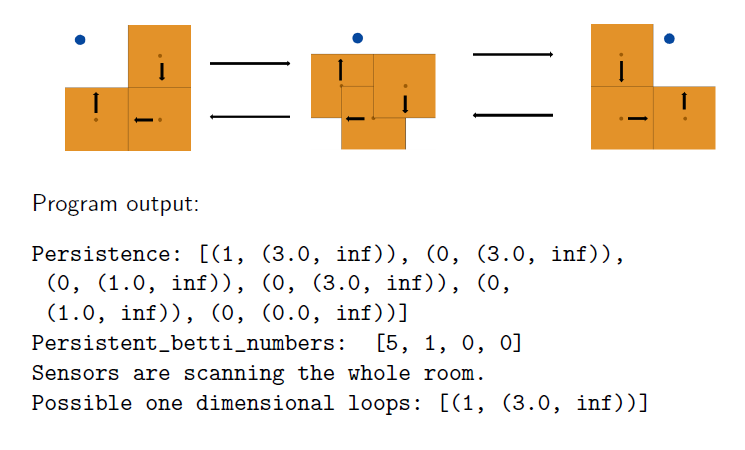
\includegraphics[width=1\textwidth]{our_example}
    \caption{Example of our end result for a simple case - the program output which consists of persistance intervals, persistent betti numbers and possible one dimensional loops (which means we have a path) together with the animation of the path we found randomly.}
    \label{fig:example}
\end{figure}


\section{Observation and notes}

Because we computed homology on a cubical complex, the complex remains connected also if cubes touch only at an edge of vertex. This means that our algorithm will find a solution also for problems where diagonal steps are needed. This is less realistic result as we are assuming the intruder has some volumen and is not simply a zero dimensional point that could move diagonally without being noticed by sensors. Figure \ref{fig:diag_steps} shows an example of such room. The output we get here is \\
\texttt{persistence:  [(1, (1.0, inf)), (0, (0.0, inf))] \\
persistent\_betti\_numbers:  [1, 1, 0, 0] \\
Sensors are scanning the whole room. \\
Possible one dimensional loops: [(1, (1.0, inf))]}.


\begin{figure}
    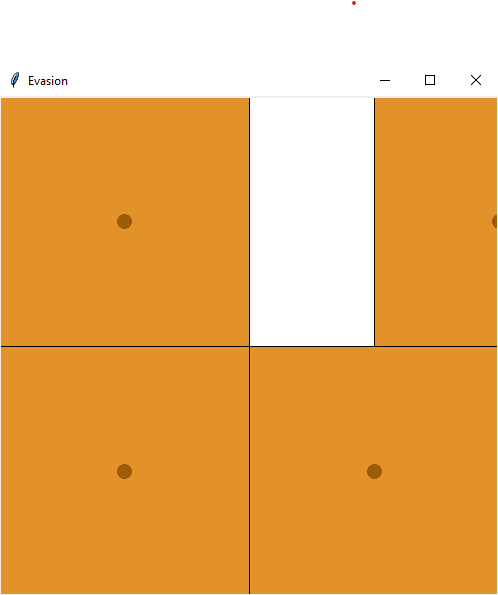
\includegraphics[width=.24\textwidth]{primer1.png}\hfill
    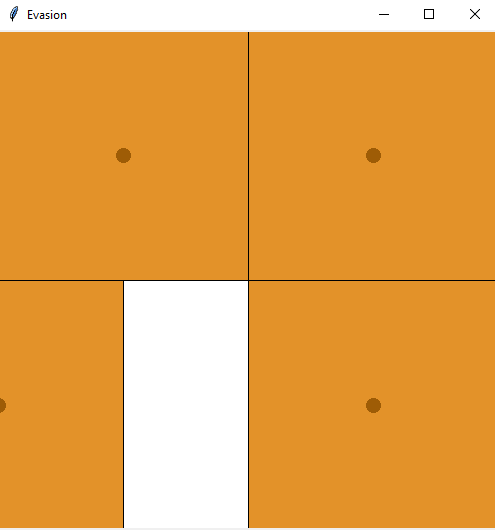
\includegraphics[width=.24\textwidth]{primer2.png}\hfill
    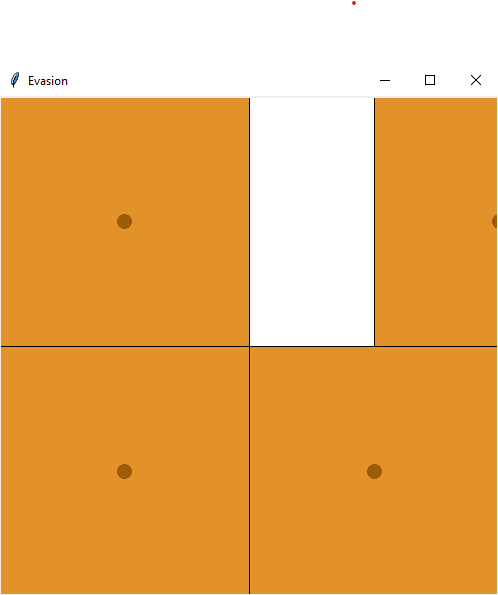
\includegraphics[width=.24\textwidth]{primer1.png}\hfill
    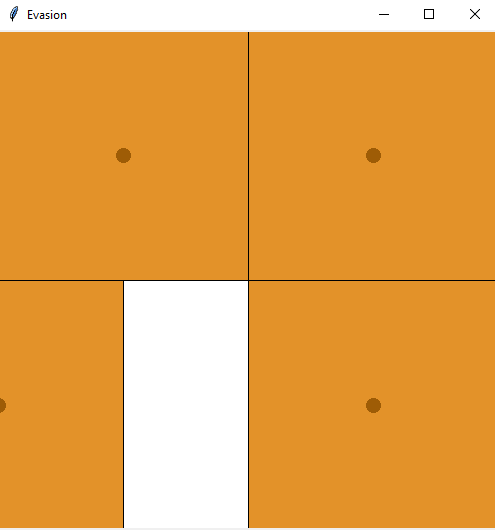
\includegraphics[width=.24\textwidth]{primer2.png}\hfill
    \caption{Example where diagonal steps are needed.}
    \label{fig:diag_steps}
\end{figure}

\section{Literature}

We used mostly the Gudhi reference manual for cubical complexes and periodic cubical complexes.






\end{document}